% physketch-doc.tex -- documentation for the physketch package
% Copyright (C) 2024-2026 Azamat Gimaev
% This file is part of the physketch package, distributed under the
% LaTeX Project Public License 1.3c or later.
\documentclass[a4paper,11pt]{article}
\usepackage[T1]{fontenc}
\usepackage{lmodern}
\usepackage[margin=2.2cm]{geometry}
\usepackage{physketch}
\usepackage[most]{tcolorbox}
\usepackage{booktabs}
\usepackage{hyperref}
\hypersetup{
  colorlinks, linkcolor=blue!50!black, urlcolor=blue!50!black,
  pdftitle={The physketch package},
  pdfauthor={Azamat Gimaev},
}

\emergencystretch=2em
\newcommand\pkg[1]{\textsf{#1}}
\newcommand\cs[1]{\texttt{\textbackslash#1}}
\newcommand\key[1]{\texttt{#1}}
\newcommand\marg[1]{\texttt{\{}\meta{#1}\texttt{\}}}
\newcommand\oarg[1]{\texttt{[}\meta{#1}\texttt{]}}
\newcommand\meta[1]{\ensuremath{\langle}\textit{#1}\ensuremath{\rangle}}

\lstdefinestyle{physketch}{
  language=[LaTeX]TeX, basicstyle=\ttfamily\small, columns=fullflexible,
  keepspaces, texcsstyle=*\color{blue!60!black},
  commentstyle=\color{black!55}\itshape,
}
\newtcblisting{example}{
  text side listing, listing options={style=physketch},
  colback=black!3, colframe=black!30, boxrule=0.4pt, arc=1mm,
  lefthand width=0.34\linewidth, sidebyside gap=4mm,
  halign lower=center}
\newtcblisting{example*}{
  text and listing, listing options={style=physketch}, unbreakable,
  halign upper=center,
  colback=black!3, colframe=black!30, boxrule=0.4pt, arc=1mm}
\newtcblisting{code}{
  listing only, listing options={style=physketch},
  colback=black!3, colframe=black!30, boxrule=0.4pt, arc=1mm}

\title{The \pkg{physketch} package\\[2pt]
  \large TikZ styles and pictures for physics drawings}
\author{Azamat Gimaev}
\date{v0.1.0 \quad 2026/10/20}

% marks an anchor in the anchor figures
\newcommand\showanchor[3][right]{%
  \fill[red] #2 circle[radius=0.8pt]
    node[#1, font=\scriptsize\ttfamily, text=red!70!black, inner sep=1.5pt] {#3};}
% the same with the label away from the point, joined by a thin line
\newcommand\showanchorat[4][right]{%
  \draw[red, ultra thin] #2 -- #3;
  \showanchor[#1]{#2}{}\path #3 node[#1, font=\scriptsize\ttfamily,
    text=red!70!black, inner sep=1.5pt] {#4};}
\newenvironment{anchors}
  {\begin{tcolorbox}[colback=white, colframe=black!30, boxrule=0.4pt, arc=1mm,
     halign=center, title={\small anchors}, coltitle=black, colbacktitle=black!8]}
  {\end{tcolorbox}}
\newcommand\swatch[1]{\tikz[baseline=-0.6ex]\fill[#1, draw=black!40] (0,-0.15) rectangle (0.6,0.25);}

\begin{document}
\maketitle

\begin{abstract}
\pkg{physketch} is a collection of TikZ styles, pictures and commands
for the drawings that appear in physics problems: fixed surfaces, mirrors,
lenses and screens, liquids and glass, springs, pulleys and weights, light
sources, field directions, and engineering-style distances. It also
encodes a consistent house style: which lines are thick, which are thin,
how large the gaps are, and what the arrow tips look like.
\end{abstract}

\tableofcontents

\section{Introduction}

\subsection{Loading}
The package consists of several parts. Load all of them at once, or only
the ones you need:
\begin{code}
\usepackage{physketch}             % everything
\usepackage{physketch.general}     % colours, materials, surfaces, vectors, distances
\usepackage{physketch.mechanics}   % bodies, springs, pulleys, weights
\usepackage{physketch.optics}      % rays, light sources, lenses, screens, mirrors
\usepackage{physketch.circuits}    % circuitikz, current sources, meters
\end{code}
Every part loads \pkg{physketch.general}. The part \pkg{physketch.circuits}
loads \pkg{circuitikz} and sets
\verb|\ctikzset{american, resistor=european, inductor=american}|.

All drawing happens inside an ordinary \texttt{tikzpicture}. The house style
(currently the arrow tip) is applied to every picture automatically:
\begin{example}
% in preamble
%\usepackage{physketch.general}
\begin{tikzpicture}
  \draw[->] (0,0) -- (2,0);
\end{tikzpicture}
\end{example}

\subsection{Settings}
Global parameters are changed with \cs{physketchset}\marg{key list}, for
example
\begin{code}
\physketchset{hatch distance=1mm, dist/offset=7mm}
\end{code}
All keys are listed in section~\ref{sec:keys}.

\subsection{General conventions}
\begin{itemize}
  \item Lines that exist only in the drawing (construction lines, distances)
    are \key{ultra thin}.
  \item Physical objects are drawn with the default line width or
    \key{thick} (vessels, surfaces, pulleys, screens).
  \item Coordinate axes and vectors use the default line width; forces are
    drawn with the style \key{force} (section~\ref{sec:forces}).
  \item Objects drawn by \cs{pulley}, \cs{piston}, \cs{lens} and
    \cs{lightsource} scale together with the picture (option \key{scale}),
    so their sizes stay consistent with the coordinates.
  \item A body resting on a surface is lifted by a small gap of
    \(0.025\,\mathrm{cm}\) to show that it can move; the same gap separates
    a piston from the walls of its vessel.
\end{itemize}

\subsection{Colours}
\begin{center}
\begin{tabular}{@{}ll@{\qquad}ll@{\qquad}ll@{}}
  \toprule
  \multicolumn{2}{@{}l}{materials} & \multicolumn{2}{l}{light rays} & \multicolumn{2}{l@{}}{bodies} \\
  \midrule
  \swatch{water} & \texttt{water} & \swatch{ray1} & \texttt{ray1} & \swatch{lightbody} & \texttt{lightbody} \\
  \swatch{ice}   & \texttt{ice}   & \swatch{ray2} & \texttt{ray2} & \swatch{body} & \texttt{body} \\
  \swatch{oil}   & \texttt{oil}   & \swatch{ray3} & \texttt{ray3} & \swatch{darkbody}  & \texttt{darkbody} \\
  \swatch{gas}   & \texttt{gas}   & & & & \\
  \swatch{glass} & \texttt{glass} & & & & \\
  \bottomrule
\end{tabular}
\end{center}
The material colours have the same names as the styles of
section~\ref{sec:materials}: \verb|\draw[water]| applies the style (a
semi-transparent fill), while \verb|fill=water!50| or \verb|draw=water| use
the colour. All colours can be redefined with \cs{definecolor} or
\cs{colorlet}.

\section{General styles}

\subsection{Fixed surfaces}
A fixed body (floor, wall, ceiling, support) is drawn with \key{surface}: a
\key{thick} line hatched on the right-hand side of the path direction.
\key{surface'} hatches the left-hand side. So a floor is drawn from left to
right with \key{surface}, a ceiling from left to right with \key{surface'}:
\begin{example}
% in preamble
%\usepackage{physketch.general}
\begin{tikzpicture}
  \draw[surface] (0,0) -- (3,0);      % floor
  \draw[surface'] (0,2) -- (3,2);     % ceiling
  \draw[surface] (-0.5,2) -- (-0.5,0); % left wall
  \draw[surface] (3.5,0) -- (3.5,2);  % right wall
\end{tikzpicture}
\end{example}
The hatching ends exactly at the ends of the path and runs continuously
along polylines (the corners are cut along their bisectors) and curves;
\verb|\fill[surface]| fills a whole area with hatching:
\begin{example}
% in preamble
%\usepackage{physketch.mechanics}
\begin{tikzpicture}
  \draw[surface] (0,1) -- (1,1) -- (1,0.4)
    -- (2.5,0.4) -- (3.5,1.4);
  \draw[surface] (0,-0.2)
    arc[start angle=180, end angle=360,
        radius=1.2] -- (3.5,-0.2);
  \draw[body]
    (1.2,-1.25) circle[radius=0.15];
  \fill[surface] (0,-2.5) rectangle (3.5,-2);
\end{tikzpicture}
\end{example}
The keys \key{hatch distance}, \key{hatch depth} and \key{hatch angle}
change the hatching of one path, for example
\verb|\draw[surface, hatch angle=-45]|.

\subsection{Materials}\label{sec:materials}
\key{water}, \key{ice}, \key{oil}, \key{gas} and \key{glass} fill an area
with a semi-transparent colour.
\begin{example}
% in preamble
%\usepackage{physketch.mechanics}
\begin{tikzpicture}
  \fill[water] (0,0) rectangle ++(2,-2.5);
  \piston[width=1.95cm]{(1,0.05)}
  \draw[thick] (0,0.8) |- (2,-2.5) -- (2,0.8);
  \draw[glass] (3,-2.5) rectangle ++(1,2);
\end{tikzpicture}
\end{example}
\begin{tcolorbox}[colback=black!3, colframe=black!30, boxrule=0.4pt, arc=1mm]
\centering
\begin{tikzpicture}
  \foreach \m [count=\i] in {water, ice, oil, gas, glass}
    \draw[\m] (2*\i,0) rectangle ++(1.5,1) node[below=2pt, midway, yshift=-0.5cm] {\small\texttt{\m}};
\end{tikzpicture}
\end{tcolorbox}

\subsection{Arrows in the middle of a path}
\key{mid arrow}\,=\,\meta{position} puts the arrow tip \verb|>| on the path
(default position \(0.6\)); \key{mid arrow'} points backwards (default
\(0.4\)).
\begin{example}
% in preamble
%\usepackage{physketch.general}
\begin{tikzpicture}
  \draw (0,0) -- ++(2.5,0);
  \draw[mid arrow] (0,-0.5) -- ++(2.5,0);
  \draw[mid arrow'] (0,-1) -- ++(2.5,0);
  \draw[mid arrow=0.3, mid arrow=0.8]
    (0,-1.5) -- ++(2.5,0);
\end{tikzpicture}
\end{example}

\subsection{Forces}\label{sec:forces}
\key{force}\,=\,\meta{radius} draws a force: a \key{thick} arrow with a dot
of the given radius (default \(0.05\,\mathrm{cm}\)) at the point of
application, the start of the path.
\begin{example}
% in preamble
%\usepackage{physketch.mechanics}
\begin{tikzpicture}
  \draw[surface] (0,0) -- (3.4,0);
  \draw[body, lifted] (1,0) rectangle ++(1.4,0.9);
  \draw[force] (1.7,0.45) -- ++(0,-1.1)
    node[right] {$m\vec g$};
  \draw[force] (1.7, 0.025) -- ++(0,1.5)
    node[right] {$\vec N$};
  \draw[force, red] (2.4,0.45) -- ++(1,0)
    node[above] {$\vec F$};
\end{tikzpicture}
\end{example}

\subsection{Vectors perpendicular to the plane}
The pics \texttt{field in} and \texttt{field out} show a vector (a field, a
current, a velocity, \ldots) perpendicular to the drawing plane, directed
into or out of it. A named pic provides the coordinate \texttt{-center}.
\begin{example}
% in preamble
%\usepackage{physketch.general}
\begin{tikzpicture}
  \foreach \x in {0,0.5,1} \pic at (\x,0) {field in};
  \foreach \x in {2,2.5,3} \pic at (\x,0) {field out};
  \node[below=2mm] at (0.5,0) {$\vec B$};
  \node[below=2mm] at (2.5,0) {$\vec v$};
\end{tikzpicture}
\end{example}

\subsection{Rotation arrows}
\verb|\rotation[|\meta{options}\verb|]{|\meta{centre}\verb|}| draws an arc
with an arrow around \meta{centre}, for an angular velocity or a rotation.
The options are
\begin{description}
  \item[\key{radius}\,=\,\meta{length}] the radius of the arc (default
    \(3\,\mathrm{mm}\));
  \item[\key{start}\,=\,\meta{angle}, \key{end}\,=\,\meta{angle}] where the
    arc starts and ends, counterclockwise (default \(45\) and \(315\));
  \item[\key{ccw}, \key{cw}] the direction of the rotation (default
    \key{ccw}): the arrow is at the end or at the start of the arc;
  \item[\key{tilt}\,=\,\meta{factor}] squeeze the arc vertically: \(1\)
    (default) is a rotation in the plane of the drawing, about \(0.35\) is a
    rotation about a vertical axis seen from the side;
  \item[\key{l}\,=\,\meta{text}] the label, put outside the arc at the angle
    \key{label angle} (default \(0\), to the right);
\end{description}
other options, like a colour, go to the arc.
\begin{example}
% in preamble
%\usepackage{physketch.general}
\begin{tikzpicture}
  \rotation{(0,0)}
  \rotation[cw, l=$\omega$]{(1,0)}
  \rotation[radius=5mm, start=-60, end=200]
    {(2.5,0)}
  \draw[dash dot, ultra thin]
    (4,-0.8) -- (4,0.8);
  \rotation[tilt=0.35, l=$\omega$]{(4,0.4)}
\end{tikzpicture}
\end{example}

\subsection{Distances}
\verb|\dist[|\meta{options}\verb|] |\meta{A}\verb| -- |\meta{B}\verb|;| is
written like a TikZ path. It draws two extension lines from the points
\meta{A} and \meta{B}, a dimension line with arrows at both ends and the
label given by the option \key{l}. By default the extension lines are
perpendicular to \(AB\) and point to the left of the direction from \(A\) to
\(B\) (walking from \(A\) to \(B\), the dimension line is on your left); a
negative \key{offset} moves the dimension line to the other side.
\begin{example}
% in preamble
%\usepackage{physketch.general}
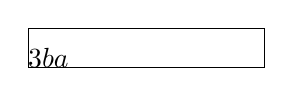
\begin{tikzpicture}
  \draw (0,0) rectangle (3,0.5);
  \dist[l=$3$~cm] (0,0.5) -- (3,0.5);
  \dist[outside, l=$b$] (0,0) -- (0,0.5);
  \dist[offset=-5mm, l=$a$] (0,0) -- (3,0);
\end{tikzpicture}
\end{example}

The options of \cs{dist} are
\begin{description}
  \item[\key{l}\,=\,\meta{text}] the label, on the outer side of the
    dimension line;
  \item[\key{l\_}\,=\,\meta{text}] the label on the inner side, between the
    dimension line and the object;
  \item[\key{pos}\,=\,\meta{fraction}] the position of the label along the
    dimension line (default \(0.5\), the middle);
  \item[\key{offset}\,=\,\meta{length}] distance from the points to the
    dimension line (default \(5\,\mathrm{mm}\));
  \item[\key{overshoot}\,=\,\meta{length}] how far the extension lines go
    beyond the dimension line (default \(1\,\mathrm{mm}\));
  \item[\key{gap}\,=\,\meta{length}] gap between a point and its extension
    line (default \(0\));
  \item[\key{direction}\,=\,\meta{angle}] draw the extension lines in a fixed
    direction instead of perpendicular to \(AB\); useful to measure a
    horizontal or vertical distance between points at different heights;
  \item[\key{outside}, \key{inside}] for small distances, \key{outside} puts
    two short arrows outside the extension lines;
  \item[\key{outside length}\,=\,\meta{length}] the length of these arrows
    (default \(2\,\mathrm{mm}\));
  \item[\key{label style}\,=\,\meta{options}, \key{line style}\,=\,\meta{options}]
    extra TikZ options for the label and for all lines.
\end{description}
Any other key is passed to TikZ and applies to the whole distance (for
example a colour). The styles \texttt{physketch/dist line},
\texttt{physketch/dist extension} and \texttt{physketch/dist label} can be
changed globally with \cs{tikzset}.

\begin{example}
% in preamble
%\usepackage{physketch.general}
\begin{tikzpicture}
  \draw[surface] (-0.3,0) -- (3,0);
  \draw (0,0) -- (2.6,1.3);
  \dist[direction=0, offset=3.5mm, l=$h$]
    (2.6,0) -- (2.6,1.3);
  \dist[offset=4mm, red, l=$\ell$, pos=0.3,
    label style={font=\small}]
    (0,0) -- (2.6,1.3);
  \dist[offset=-12mm, l_=$d$] (0,0) -- (3,0);
\end{tikzpicture}
\end{example}

\subsection{Angles}
\verb|\angledist[|\meta{options}\verb|] |\meta{A}\verb| -- |\meta{O}\verb| -- |\meta{B}\verb|;|
draws an arc around the vertex \meta{O} from the ray \(OA\) to the ray
\(OB\), counterclockwise (as in the TikZ library \texttt{angles}); to mark
the other angle, swap \meta{A} and \meta{B}. The points can be coordinates
or names. The options are
\begin{description}
  \item[\key{l}\,=\,\meta{text}] the label, outside the arc;
  \item[\key{l\_}\,=\,\meta{text}] the label inside the arc;
  \item[\key{pos}\,=\,\meta{fraction}] the position of the label along the
    arc (default \(0.5\), the middle);
  \item[\key{radius}\,=\,\meta{length}] the radius of the arc (default
    \(0.75\,\mathrm{cm}\));
  \item[\key{label distance}\,=\,\meta{length}] the gap between the arc and
    the label (default \(1\,\mathrm{mm}\)); the label touches the arc with
    its side, so it never covers the arc whatever the radius;
  \item[\key{label radius}\,=\,\meta{length}] put the centre of the label at
    this distance from the vertex instead;
  \item[\key{label style}\,=\,\meta{options}] extra TikZ options for the
    label.
\end{description}
Other options, like \key{double} or a colour, go to TikZ.
\begin{example}
% in preamble
%\usepackage{physketch.general}
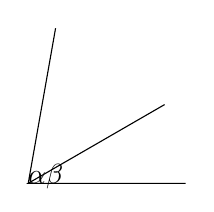
\begin{tikzpicture}
  \coordinate (O) at (0,0);
  \coordinate (A) at (2,0);
  \coordinate (B) at (30:2);
  \coordinate (C) at (80:2);
  \draw (A) -- (O) -- (B) (O) -- (C);
  \angledist[l=$\alpha$] (A) -- (O) -- (B);
  \angledist[double=yellow!20, radius=0.9cm,
    l=$\beta$] (B) -- (O) -- (C);
\end{tikzpicture}
\end{example}
\begin{example}
% in preamble
%\usepackage{physketch.general}
\begin{tikzpicture}
  \draw (0,0) -- (2.5,0) -- (1.2,1.6) -- cycle;
  \angledist[l_=$\varphi$, radius=1cm]
    (2.5,0) -- (0,0) -- (1.2,1.6);
  \angledist[l=$\psi$, radius=4mm]
    (1.2,1.6) -- (2.5,0) -- (0,0);
\end{tikzpicture}
\end{example}

\section{Mechanics}
\emph{Part \pkg{physketch.mechanics}.}

\subsection{Bodies}
\key{body} draws a body filled with the grey colour \texttt{body};
\key{light body} and \key{dark body} use the colours \texttt{lightbody} and
\texttt{darkbody}. A white body is drawn with a plain \cs{draw}.
\key{piston} is the same as \key{body} (for pistons of other shapes; see
also \cs{piston}). \key{lifted}\,=\,\meta{angle} shifts the object by the
gap in the given direction (default \(90\), i.e.\ up).
\begin{example}
% in preamble
%\usepackage{physketch.mechanics}
\begin{tikzpicture}
  \draw[surface] (-0.5,0) -- (4.5,0);
  \draw[lifted] (0,0) rectangle ++(1,0.8);
  \draw[light body, lifted] (1.5,0) rectangle ++(1,0.8);
  \draw[body, lifted] (3,0) rectangle ++(1,0.8);
\end{tikzpicture}
\end{example}

\subsection{Springs}
\key{spring} turns a straight path into a spring. Its value is a list of
options:
\begin{description}
  \item[\key{segment length}\,=\,\meta{length}] the length of one coil
    (default \(2\,\mathrm{mm}\));
  \item[\key{coils}\,=\,\meta{number}] the number of coils instead; the
    coil length is then computed from the length of the path;
  \item[\key{amplitude}\,=\,\meta{length}] half of the width of the spring
    (default \(2\,\mathrm{mm}\));
  \item[\key{ends}\,=\,\meta{length}] the straight parts at both ends
    (default \(1\,\mathrm{mm}\));
\end{description}
\begin{example}
% in preamble
%\usepackage{physketch.mechanics}
\begin{tikzpicture}
  \draw[spring] (0,0) -- (3,0);
  \draw[spring={coils=6}] (0,-0.6) -- (3,-0.6);
  \draw[spring={amplitude=1mm,
    segment length=2mm, ends=7mm}]
    (0,-1.2) -- (3,-1.2);
\end{tikzpicture}
\end{example}
\pkg{circuitikz} has its own \key{spring} (a mechanical bipole). When
\pkg{physketch.circuits} is loaded, it is available as \key{circuit spring}:
\verb|\draw (0,0) to[circuit spring] (2,0);|.

\subsection{Pistons}
\cs{piston}\oarg{options}\marg{centre} draws a piston: a grey plate centred
at \meta{centre} with a rod. The options are
\begin{description}
  \item[\key{name}\,=\,\meta{name}] the name of the piston;
  \item[\key{width}\,=\,\meta{length}] the width of the plate (default
    \(2\,\mathrm{cm}\)); by the conventions it is the width of the vessel
    minus two gaps of \(0.025\,\mathrm{cm}\);
  \item[\key{thickness}\,=\,\meta{length}] the thickness of the plate
    (default \(1\,\mathrm{mm}\));
  \item[\key{rod}\,=\,\meta{length}] the length of the rod (default
    \(1\,\mathrm{cm}\); \(0\) draws no rod);
  \item[\key{rod side}\,=\,\meta{anchor}] where the rod starts: \key{north}
    (default), \key{south}, \key{east} or \key{west};
\end{description}
other options, like \key{rotate} or \key{fill}, go to the plate.
\begin{example}
% in preamble
%\usepackage{physketch.mechanics}
\begin{tikzpicture}
  \fill[gas] (0,0) rectangle (2,1.5);
  \draw[thick] (0,2.6) |- (2,0) -- (2,2.6);
  \piston[name=P, width=1.95cm]{(1,1.55)}
  \draw[force] (P-rod) -- ++(0,0.5) node[right] {$\vec F$};
  \piston[rotate=90, width=1cm, rod side=south]
    {(3,0.8)}
\end{tikzpicture}
\end{example}
\begin{anchors}
\begin{tikzpicture}
  \piston[name=P, width=4cm, thickness=1cm, rod=1.2cm]{(0,0)}
  \showanchor[above]{(P-rod)}{P-rod}
  \showanchor[above left]{(P.north west)}{P.north west}
  \showanchor[above right]{(P.north east)}{P.north east}
  \showanchor[left]{(P.west)}{P.west}
  \showanchor[right]{(P.east)}{P.east}
  \showanchor[below]{(P.south)}{P.south}
  \showanchor[below left]{(P.south west)}{P.south west}
  \showanchor[below right]{(P.south east)}{P.south east}
\end{tikzpicture}
\end{anchors}

\subsection{Pulleys}
\cs{pulley}\oarg{options}\marg{centre} draws a pulley. The options are
\begin{description}
  \item[\key{name}\,=\,\meta{name}] the name of the pulley;
  \item[\key{outer}\,=\,\meta{length}] the radius of the wheel (default
    \(0.5\,\mathrm{cm}\));
  \item[\key{inner}\,=\,\meta{length}] the radius of the axle (default
    \(0.05\,\mathrm{cm}\));
\end{description}
other options, like \key{fill}, go to the wheel. A pulley named \texttt{p}
is a circular node: its border anchors \texttt{p.north}, \texttt{p.west},
\texttt{p.-45}, \ldots\ (any angle) lie on the wheel. The axle is the node
\texttt{p-center}; a line drawn from \texttt{(p-center)} starts at the edge
of the axle, so the axle stays clean.
\begin{example}
% in preamble
%\usepackage{physketch.mechanics}
\begin{tikzpicture}
  \draw[surface'] (-1,2) -- (1,2);
  \pulley[name=p, outer=0.6cm]{(0,0)}
  \draw (p-center) -- (0,2);
  \draw (p.west) -- ++(0,-1.4) pic {weight};
  \draw (p.45) -- ++(-45:1);
  \draw[force, red] (p.45) ++(-45:1)
    -- ++(-45:0.8) node[right, black] {$\vec F$};
\end{tikzpicture}
\end{example}
\begin{anchors}
\begin{tikzpicture}
  \pulley[name=p, outer=1.2cm, inner=0.1cm]{(0,0)}
  \showanchor[above]{(p.north)}{p.north}
  \showanchor[below]{(p.south)}{p.south}
  \showanchor[left]{(p.west)}{p.west}
  \showanchor[right]{(p.east)}{p.east}
  \showanchor[above right]{(p.45)}{p.45}
  \showanchor[below right]{(p.-45)}{p.-45}
  \showanchor[above left]{(p.150)}{p.150}
  \showanchor[below]{(p-center.south)}{p-center}
\end{tikzpicture}
\end{anchors}

\subsection{Rods divided into equal parts}
\key{rod}\,=\,\meta{options} turns a straight path into a bar made of
alternating light and dark parts of equal length, which shows the lever arms
in statics problems. The options are
\begin{description}
  \item[\key{segments}\,=\,\meta{number}] the number of parts (default
    \(10\));
  \item[\key{width}\,=\,\meta{length}] the width of the bar (default
    \(1.5\,\mathrm{mm}\));
  \item[\key{start light}, \key{start dark}] the colour of the first part
    (default \key{start light});
  \item[\key{light}\,=\,\meta{colour}, \key{dark}\,=\,\meta{colour}] the
    colours of the parts (default \texttt{white} and \texttt{darkbody});
  \item[\key{name}\,=\,\meta{name}] a rod named \texttt{R} provides the
    coordinates \texttt{R-}\meta{i}, \(i=0,\ldots,\)\key{segments}, on its axis
    at the borders of the parts, and \texttt{R-}\meta{i}\texttt{-top},
    \texttt{R-}\meta{i}\texttt{-bottom} on its sides (\texttt{top} is on the
    left of the direction of the path).
\end{description}
\begin{example*}
% in preamble
%\usepackage{physketch.mechanics}
\begin{tikzpicture}
  \draw[rod={segments=12, name=R}] (0,0) -- (6,0);
  \pic at (R-2-bottom) {fulcrum};
  \draw (R-1-bottom) -- ++(0,-1.2);
  \draw (R-3-bottom) -- ++(0,-1.2);
  \pulley[name=p]{(1,-1.2)}
  \draw (p-center) -- ++(0,-1.2) node[draw, below, minimum size=3mm] {};
  \draw (R-12-bottom) -- ++(0,-0.8) node[draw, below, minimum size=3mm] {};
  \draw[->] (6.5,-0.6) -- ++(0,-0.8) node[midway, right] {$v$};
\end{tikzpicture}
\end{example*}
\begin{anchors}
\begin{tikzpicture}
  \draw[rod={segments=4, width=8mm, name=R}] (0,0) -- (8,0);
  \foreach \i in {0,...,4} {
    \fill[red] (R-\i) circle[radius=0.8pt];
    \showanchor[above]{(R-\i-top)}{R-\i-top}
    \showanchor[below]{(R-\i-bottom)}{R-\i-bottom}
  }
  \showanchorat[left]{(R-0)}{(-0.6,0)}{R-0}
  \showanchorat[right]{(R-4)}{(8.6,0)}{R-4}
\end{tikzpicture}
\end{anchors}

\subsection{Pictures}
The TikZ \emph{pics} \texttt{fulcrum} (a point of support: its apex is at
the origin and the hatched base below; \key{rotate}\,=\,\(180\) gives a point
of suspension), \texttt{weight} (standing on its base) and \texttt{nut} are
placed with \verb|\pic at (x,y) {name};|. A named pic,
\verb|\pic (w) at ... {weight};|, provides the coordinates shown below.
\begin{example}
% in preamble
%\usepackage{physketch.mechanics}
\begin{tikzpicture}
  \draw[thick] (-1,0) -- (1,0);
  \pic at (0,0) {fulcrum};
  \pic (h) [rotate=180] at (2,0.5) {fulcrum};
  \draw (h-center) -- (2,-0.7) pic (w) {weight};
  \pic at (0,-1) {nut};
\end{tikzpicture}
\end{example}
\begin{anchors}
\begin{tikzpicture}
  \pic[scale=3] (f) at (0,0) {fulcrum};
  \showanchor[above]{(f-center)}{f-center}
  \showanchorat{(f-base)}{($(f-base)+(1.2,0.3)$)}{f-base}
  \pic[scale=3] (w) at (3,-0.6) {weight};
  \showanchorat{(w-center)}{($(w-center)+(1.2,0)$)}{w-center}
  \showanchor[right=2pt]{(w-top)}{w-top}
  \pic[scale=3] (n) at (7.6,0) {nut};
  \showanchorat{(n-center)}{($(n-center)+(1.6,-0.6)$)}{n-center}
\end{tikzpicture}
\end{anchors}

\section{Optics}
\emph{Part \pkg{physketch.optics}.}

\subsection{Rays}
\key{ray}\,=\,\meta{n} draws a light ray in the colour
\texttt{ray}\meta{n}, where \meta{n} is 1 (yellow, the default), 2 (red) or
3 (blue). \key{virtual ray}\,=\,\meta{n} draws its continuation dashed, and
\key{optical axis} is a thin dash-dotted line.

\key{object} draws an object (an arrow from \(A\) to \(B\)) and
\key{virtual object} its virtual image, dashed.
\begin{example}
% in preamble
%\usepackage{physketch.optics}
\begin{tikzpicture}
  \draw[optical axis] (-0.5,0) -- (3.5,0);
  \draw[object] (0,0) -- ++(0,0.8)
    node[left] {$B$};
  \node[below] at (0,0) {$A$};
  \draw[virtual object] (2.5,0) -- ++(0,1.2)
    node[left] {$B'$};
\end{tikzpicture}
\end{example}

\subsection{Light sources}
\cs{lightsource}\oarg{options}\marg{position} draws a point light source.
The options are
\begin{description}
  \item[\key{name}\,=\,\meta{name}] the name of the source;
  \item[\key{radius}\,=\,\meta{length}] the length of the rays of the symbol
    (default \(0.15\,\mathrm{cm}\));
  \item[\key{halo}\,=\,\meta{length}] the radius of the halo around the
    source, from its centre (default \(0.2\,\mathrm{cm}\));
  \item[\key{fill}\,=\,\meta{colour}] the colour of the halo (default
    \texttt{white}).
\end{description}
A source named \texttt{S} is a circular node of radius \key{halo}. Lines
drawn from \texttt{(S)} start at the edge of the halo, so rays never cross
the source; \texttt{S.center} is the source itself. Labels of light sources
are placed \(0.2\,\mathrm{cm}\) away from them.
\begin{example}
% in preamble
%\usepackage{physketch.optics}
\begin{tikzpicture}
  \lightsource[name=S]{(0,0)}
  \node[above=0.2cm] at (S) {$S$};
  \foreach \a in {-30,0,30} \draw[ray] (S) -- (\a:2);
  \lightsource[fill=ray1!30]{(0,-1)}
\end{tikzpicture}
\end{example}
\begin{anchors}
\begin{tikzpicture}[scale=1]
  \lightsource[name=S, halo=1cm, radius=0.6cm]{(0,0)}
  \draw[ultra thin, dashed] (S.center) circle[radius=1cm];
  \showanchorat[right]{(S.center)}{(1.8,-0.9)}{S.center}
  \showanchor[right]{(S.east)}{S.east}
  \showanchor[above]{(S.north)}{S.north}
  \showanchor[above right]{(S.45)}{S.45}
  \showanchor[left]{(S.west)}{S.west}
\end{tikzpicture}
\end{anchors}

\subsection{Lenses}
\cs{lens}\oarg{options}\marg{centre} draws a thin lens. The options are
\begin{description}
  \item[\key{name}\,=\,\meta{name}] the name of the lens;
  \item[\key{height}\,=\,\meta{length}] the height of the lens (default
    \(3\,\mathrm{cm}\));
  \item[\key{converging}, \key{diverging}] the kind of lens (default
    \key{converging});
\end{description}
other options, like \key{rotate}, go to the node. A lens named \texttt{L} is
a node of zero width. The lines are drawn with the styles
\texttt{physketch/lens} and \texttt{physketch/diverging lens}, which can be
changed with \cs{tikzset}.
\begin{example}
% in preamble
%\usepackage{physketch.optics}
\begin{tikzpicture}
  \draw[optical axis] (-2.2,0) -- (2.4,0);
  \lens[name=L]{(0,0)}
  \lightsource[name=S]{(-2,0.6)}
  \draw[ray, mid arrow] (S) -- (0,0.6) -- (2,-0.6);
  \draw[ray=2, mid arrow] (S) -- (0,0) -- (2,-0.6);
  \draw[virtual ray] (0,0.6) -- (-1,1.2);
  \lens[diverging, height=2cm]{(2.4,0)}
\end{tikzpicture}
\end{example}
\begin{anchors}
\begin{tikzpicture}
  \draw[optical axis] (-2.6,0) -- (2.6,0);
  \lens[name=L, height=2.4cm]{(0,0)}
  \showanchor[right]{(L.north)}{L.north}
  \showanchor[above right]{(L.center)}{L.center}
  \showanchor[right]{(L.south)}{L.south}
  \lens[name=M, height=2.4cm, diverging, rotate=0]{(4,0)}
  \showanchor[right]{(M.center)}{M.center}
  \showanchor[right]{(M.north)}{M.north}
  \showanchor[right]{(M.south)}{M.south}
\end{tikzpicture}
\end{anchors}

\subsection{Screens}
\key{screen} is a \key{thick} line with sparse hatching on the right-hand
side of the path direction; \key{screen'} puts it on the left-hand side. The
spacing of the hatching is the key \key{screen distance}. Straight and curved
paths both work.
\begin{example}
% in preamble
%\usepackage{physketch.optics}
\begin{tikzpicture}
  \draw[screen] (0,2) -- (0,0);
  \draw[screen'] (0.8,2) -- (0.8,0);
  \draw[screen'] (1.6,0) -- (3.6,0);
  \draw[screen] (1.8,0.6) arc[start angle=180,
    end angle=90, radius=1.4];
\end{tikzpicture}
\end{example}

\subsection{Mirrors}
\key{mirror} is a \key{thick} line with a grey gradient on the right-hand
side of the path direction, fading away from the line; \key{mirror'} puts it
on the left-hand side. The width of the gradient is the key \key{mirror
width}. Straight and curved paths both work.
\begin{example}
% in preamble
%\usepackage{physketch.optics}
\begin{tikzpicture}
  \draw[mirror] (0,2) -- (0,0);
  \draw[mirror] (1.2,1.9)
    arc[start angle=23.6, end angle=-23.6, radius=4.8];
  \draw[mirror'] (2.4,1.9)
    arc[start angle=156.4, end angle=203.6, radius=4.8];
  \draw[mirror'] (3,0) -- (4,0);
\end{tikzpicture}
\end{example}

\section{Circuits}
\emph{Part \pkg{physketch.circuits}.} It loads \pkg{circuitikz} with
American symbols except for European resistors; all \pkg{circuitikz}
components are available as usual. The vectors \texttt{field in} and
\texttt{field out} come from \pkg{physketch.general}.
\begin{example}
% in preamble
%\usepackage{physketch.circuits}
\begin{tikzpicture}
  \draw (0,0) to[battery1, l=$\mathcal{E}$] (0,2.5)
    to[R=$R_1$] (4,2.5) to[C=$C$] (4,0)
    to[L=$L$] (0,0);
  \draw (4,0) node[ground] {};
  \foreach \x in {1.4,2,2.6}
    \pic at (\x,1.25) {field in};
\end{tikzpicture}
\end{example}

\subsection{Current sources}
Besides the \pkg{circuitikz} current source \key{I} (an arrow in a circle),
the package defines its second variant \key{I'} (long name \key{current
source'}): two chevrons in a circle. With \key{invert} they point the other
way.
\begin{example}
% in preamble
%\usepackage{physketch.circuits}
\begin{tikzpicture}
  \draw (0,0) to[I] (2,0);
  \draw (0,-1.5) to[I'] ++(2,0);
  \draw (0,-3) to[I', invert, l_=$I_0$] ++(2,0);
\end{tikzpicture}
\end{example}

\subsection{Meters}
\key{ammeter}, \key{voltmeter} and \key{ohmmeter} draw a round meter with a
bold letter that stays upright. An optional index, like \verb|voltmeter=2|,
is written as a subscript; the letter together with its index is centred in
the circle.
\begin{example}
% in preamble
%\usepackage{physketch.circuits}
\begin{tikzpicture}
  \draw (0,0) to[ammeter] (1.4,0)
    to[ammeter=1] (2.8,0)
    to[ammeter=2] (4.2,0);
  \draw (0,-1) to[voltmeter] (1.4,-1)
    to[voltmeter=2] (2.8,-1)
    to[ohmmeter] (4.2,-1);
\end{tikzpicture}
\end{example}

\section{Gallery}
\begin{example*}
% in preamble
%\usepackage{physketch.optics}
\begin{tikzpicture}
  \lightsource[name=A]{(0,0)}
  \node[above=0.2cm] at (A) {$A$};
  \fill[black!10] (-5,-2.5) -- (-3,-1.5) -- (-3,-2) -- (-1,-2) -- (-1.25,-2.5);
  \draw[glass] (-3,-2) rectangle ++(2,0.5);
  \draw[surface] (-6,-2.5) -- (1,-2.5);

  \dist[offset=-5mm, l=$L$] (-5,-2.5) -- (-1.25,-2.5);
  \dist[l=$a$] (-3,-1.5) -- (-1,-1.5);
  \dist[offset=-5mm, outside, l=$b$] (-3,-1.5) -- (-3,-2);

  \draw[ultra thin] (-1,-2) -- (0.5,-2);
  \dist[offset=0pt, overshoot=0pt, l=$H_0-h$] (A.south) -- (0,-2);
  \dist[offset=0pt, overshoot=0pt, l=$h$] (0,-2) -- (0,-2.5);
\end{tikzpicture}
\end{example*}

\begin{example*}
% in preamble
%\usepackage{physketch.mechanics}
\begin{tikzpicture}
  \draw[thick, fill=lightbody] (-3,-3) rectangle (3,3) node[above left] {$m_1$};
  \draw[force] (0,3) -- ++(0,1) node[right] {$\vec F$};
  \draw[spring={coils=7, amplitude=1mm}] (0,3) -- (0,1.5)
    node[midway, right=0.1cm] {$k_1$};
  \draw[body] (-1,1.5) rectangle (1,0.5) node[midway] {$m_2$};
  \draw[spring={coils=9, amplitude=1mm}] (0,0.5) -- (0,-1)
    node[midway, right=0.1cm] {$k_2$};
  \draw[body] (-1,-1) rectangle (1,-2) node[midway] {$m_3$};
  \draw[->] (3.5,0.5) -- (3.5,-0.5) node[midway, right] {$g$};
\end{tikzpicture}
\end{example*}

\section{Reference}\label{sec:keys}
\subsection{Global keys}
These keys live in \texttt{/physketch} and are set with \cs{physketchset}.
\begin{center}
\begin{tabular}{lll}
  \toprule
  key & default & meaning \\
  \midrule
  \key{gap} & 0.25mm & gap used by \key{lifted} \\
  \key{hatch distance} & 0.74mm & spacing of the hatching \\
  \key{hatch depth} & 1mm & width of the hatched band \\
  \key{hatch angle} & 45 & angle of the hatching strokes \\
  \key{hatch line width} & 0.4pt & line width of the hatching strokes \\
  \key{screen distance} & 1.2mm & spacing of the hatching of \key{screen} \\
  \key{mirror width} & 2mm & width of the gradient of \key{mirror} \\
  \key{dist/\meta{key}} & & defaults for \cs{dist} \\
  \key{angle/\meta{key}} & & defaults for \cs{angledist} \\
  \key{spring/\meta{key}} & & defaults for \key{spring} \\
  \key{rod/\meta{key}} & & defaults for \key{rod} \\
  \key{piston/\meta{key}} & & defaults for \cs{piston} \\
  \key{pulley/\meta{key}} & & defaults for \cs{pulley} \\
  \key{light source/\meta{key}} & & defaults for \cs{lightsource} \\
  \key{lens/\meta{key}} & & defaults for \cs{lens} \\
  \key{rotation/\meta{key}} & & defaults for \cs{rotation} \\
  \bottomrule
\end{tabular}
\end{center}

\subsection{Commands}
\begin{center}\small
\begin{tabular}{lll}
  \toprule
  command & part & purpose \\
  \midrule
  \cs{physketchset}\marg{keys} & general & settings \\
  \verb|\dist[|\meta{options}\verb|] |\meta{A}\verb| -- |\meta{B}\verb|;| & general & distances \\
  \verb|\angledist[|\meta{options}\verb|] |\meta{A}\verb| -- |\meta{O}\verb| -- |\meta{B}\verb|;| & general & angles \\
  \cs{piston}\oarg{options}\marg{centre} & mechanics & pistons \\
  \cs{pulley}\oarg{options}\marg{centre} & mechanics & pulleys \\
  \cs{lightsource}\oarg{options}\marg{position} & optics & light sources \\
  \cs{lens}\oarg{options}\marg{centre} & optics & lenses \\
  \cs{rotation}\oarg{options}\marg{centre} & general & rotation arrows \\
  \bottomrule
\end{tabular}
\end{center}

\subsection{TikZ styles}
\begin{center}\small
\begin{tabular}{lll}
  \toprule
  style & part & purpose \\
  \midrule
  \key{surface}, \key{surface'} & general & fixed surfaces and areas \\
  \key{hatch distance}, \key{hatch depth}, \key{hatch angle} & general & local hatching settings \\
  \key{water}, \key{ice}, \key{oil}, \key{gas}, \key{glass} & general & materials \\
  \key{mid arrow}, \key{mid arrow'} & general & arrow tips on a path \\
  \key{force}\,=\,\meta{radius} & general & forces \\
  \key{body}, \key{light body}, \key{dark body}, \key{piston} & mechanics & bodies \\
  \key{lifted}\,=\,\meta{angle} & mechanics & shift by the gap \\
  \key{spring}\,=\,\meta{options} & mechanics & springs \\
  \key{rod}\,=\,\meta{options} & mechanics & rods divided into equal parts \\
  \key{ray}\,=\,\meta{n}, \key{virtual ray}\,=\,\meta{n}, \key{optical axis} & optics & rays \\
  \key{object}, \key{virtual object} & optics & objects and images \\
  \key{screen}, \key{screen'} & optics & screens \\
  \key{mirror}, \key{mirror'} & optics & mirrors \\
  \key{circuit spring} & circuits & the \pkg{circuitikz} spring \\
  \key{I'} & circuits & current source with chevrons \\
  \key{ammeter}, \key{voltmeter}, \key{ohmmeter}\,=\,\meta{index} & circuits & meters \\
  \bottomrule
\end{tabular}
\end{center}

\subsection{Pictures}
\begin{center}\small
\begin{tabular}{ll}
  \toprule
  part & pics \\
  \midrule
  general & \texttt{field in}, \texttt{field out} \\
  mechanics & \texttt{fulcrum}, \texttt{weight}, \texttt{nut} \\
  \bottomrule
\end{tabular}
\end{center}

\end{document}
